\documentclass[../mathNotesPreamble]{subfiles}

\providecommand{\relscalefact}{1.4}
\begin{document}
\relscale{\relscalefact}
  \section{2.2: Summarizing Important Features of a Numerical Distribution}
  \begin{defn*}
    When examining a distribution:
    \begin{itemize}
      \item the \textbf{center} represents the typical or most common values, and
      \item the \textbf{spread} represents the variability in the data.
    \end{itemize}
  \end{defn*}
  \begin{ex*}
    Below are the histograms containing the number of goals scored by first year NCAA female (left) and male (right) soccer players in Division III in the 2016-17 season:
  \end{ex*}
  \begin{center}
    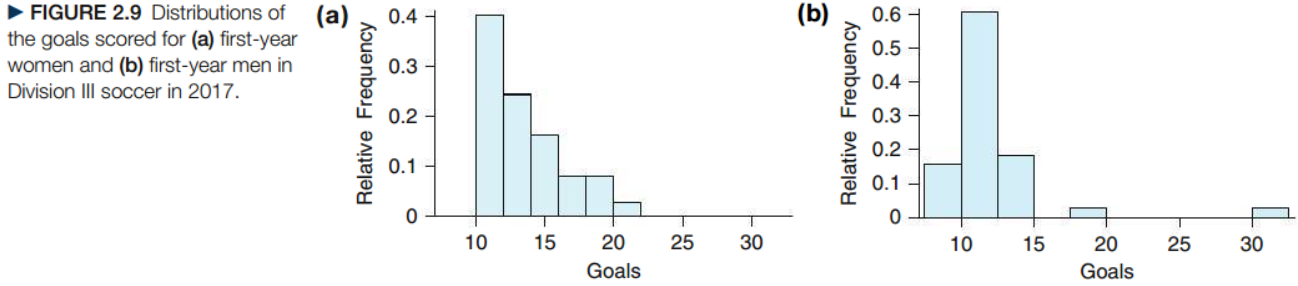
\includegraphics[width=0.975\linewidth]{images/math211_figure_2p09}
  \end{center}
  \begin{tasks}[after-item-skip=\stretch{1}, label=--](1)
    \task Are their any notable differences in the shapes?
    \task What is the approximate center for each distribution?
    \task How do the spreads compare?
  \end{tasks}
  \vspace*{\stretch{1}}
  \pagebreak

  \begin{center}
    \fbox{\parbox{0.9\linewidth}{
      Three basic characteristics to consider when examining a distribution's shape:
      \begin{enumerate}
        \item Is the distribution symmetric or skewed?
        \item How many ``mounds'' appear?
        \item Are unusually large or small values present?
      \end{enumerate}
    }}
    \vspace*{0.5\baselineskip}

    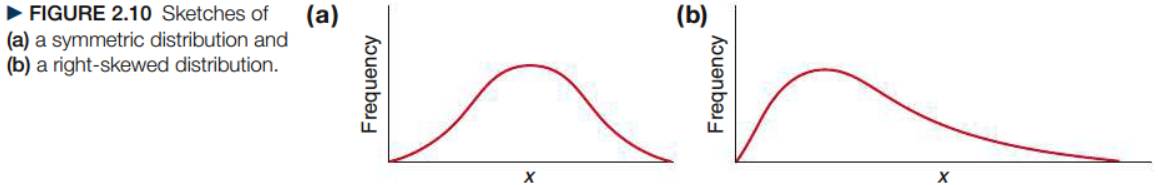
\includegraphics[width=0.95\linewidth]{images/math211_figure_2p10}
  \end{center}
  \begin{defn*}
    \begin{itemize}
      \item A \textbf{right-skewed distribution} has a ``tail'' that extends towards the right.
      \item A \textbf{left-skewed distribution} has a ``tail'' that extends towards the left.
      \item A \textbf{symmetric} distribution has ``tails'' of approximately equal size.
    \end{itemize}
  \end{defn*}
  \vspace*{\stretch{1}}
  \begin{center}
    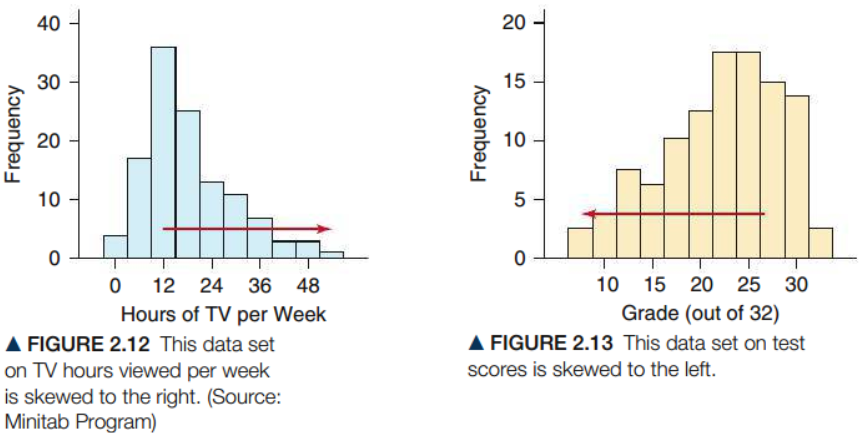
\includegraphics[width=0.725\linewidth]{images/math211_figure_2p12_2p13}
  \end{center}
  \pagebreak

  \begin{defn*}
    \begin{itemize}
      \item A \textbf{unimodal distribution} has data grouped in a single ``mound'',
      \item a \textbf{bimodal distribution} has data grouped in two ``mounds'', and
      \item a \textbf{multimodal distribution} has data grouped in more than two ``mounds''.
    \end{itemize}
  \end{defn*}
  \begin{center}
    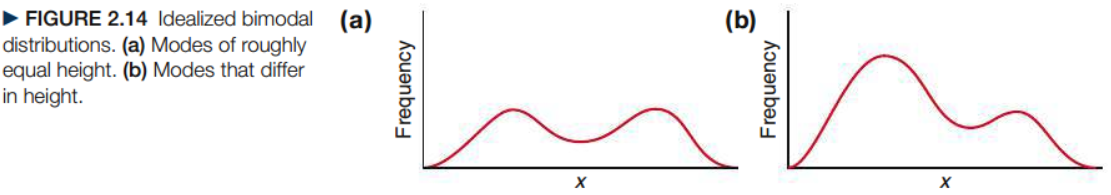
\includegraphics[width=0.95\linewidth]{images/math211_figure_2p14}
  \end{center}
  \begin{ex*}
    In a 5k/10k race where all the runners start at the same time, what do we expect the shape of the distribution of the finishing times will look like?
  \end{ex*}
  \pagebreak

  \begin{defn*}
    An \textbf{outlier} is an extreme value in a distribution of data. Outliers don't fit the pattern of the rest of the data.
  \end{defn*}
  \begin{ex*}
    Consider the distribution of exam grades. What are possible explanations of any outliers?
  \end{ex*}
  \vspace*{\stretch{1}}

  \begin{defn*}
    The most frequently occuring value is called the \textbf{mode}.
  \end{defn*}

  \noindent
  Why might the mode not be a reliable measure of center for numerical data?
  \vspace*{5\baselineskip}
  \pagebreak


  \pagebreak
\end{document}
